\documentclass{article}

\usepackage[letterpaper, margin=20mm]{geometry}
\usepackage{hyperref}
\usepackage{graphicx}
\usepackage{listings}
\usepackage{color}

\begin{document}

\pagenumbering{arabic}
\begin{center}
{\huge Android Guide}\\[0.5 cm]
{\large CS 2340, Summer 2018}\\[0.2 cm]
{\large Author: Isaac Weintraub}\\[0.2 cm]
\end{center}
\tableofcontents
\vspace{12mm}
\hrule
\vspace{6mm}

\section{Introduction}
Unlike in past semesters, Android is \textbf{NOT} required as the platform for your app - you are free to choose this or any Java (\underline{not} JavaScript)-based web framework. However, if your team would like to use Android, feel free to do so. This document outlines the basics of working with Android and creating a simple project.

\section{Getting Started}
You will develop your Android app using the Android Studio IDE. If you have used IntelliJ in CS 1332, you may find some aspects of Android Studio familiar.\\[0.2cm]
\href{https://developer.android.com/studio/}{\textbf{Download Android Studio here.}}\\[0.2cm]
Once Android Studio is installed, open it. You should see the following screen:
\begin{center}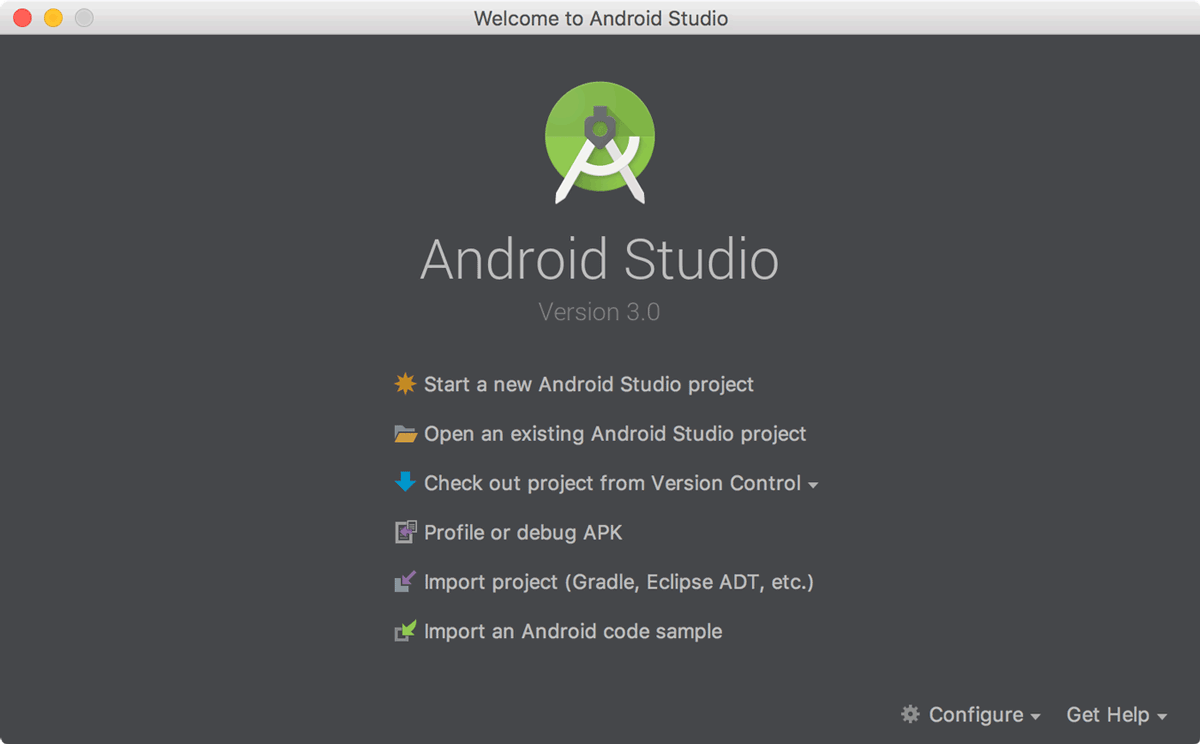
\includegraphics[width=.5\textwidth]{images/studio-open.png}\end{center}
In the window that follows, enter the name for your application, a company domain, and select a location for your project.
\begin{center}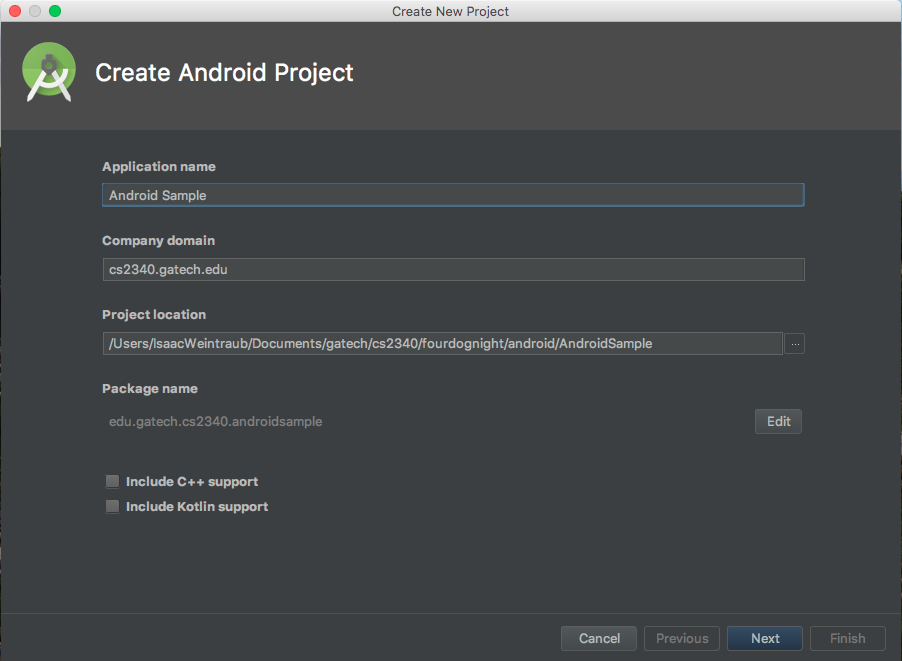
\includegraphics[width=.5\textwidth]{images/create-new.png}\end{center}
Click Next to go to the Target Android Devices screen. Leave Phone and Tablet checked. Choose the API level you want your app to target. Using a newer API level (higher number) will allow your app to use more features, but it will reduce the proportion of devices that your app is compatible with. For the purposes of CS 2340, the API level you target is not important. It is fine to leave the default value, since you can change it later if it becomes necessary to do so. Click Next again to go to the Add an Activity to Mobile screen. Select Empty Activity, and click Next. This will bring you to the Configure Activity screen. You can leave the default values here, and click Finish. The IDE will open after some processing:
\begin{center}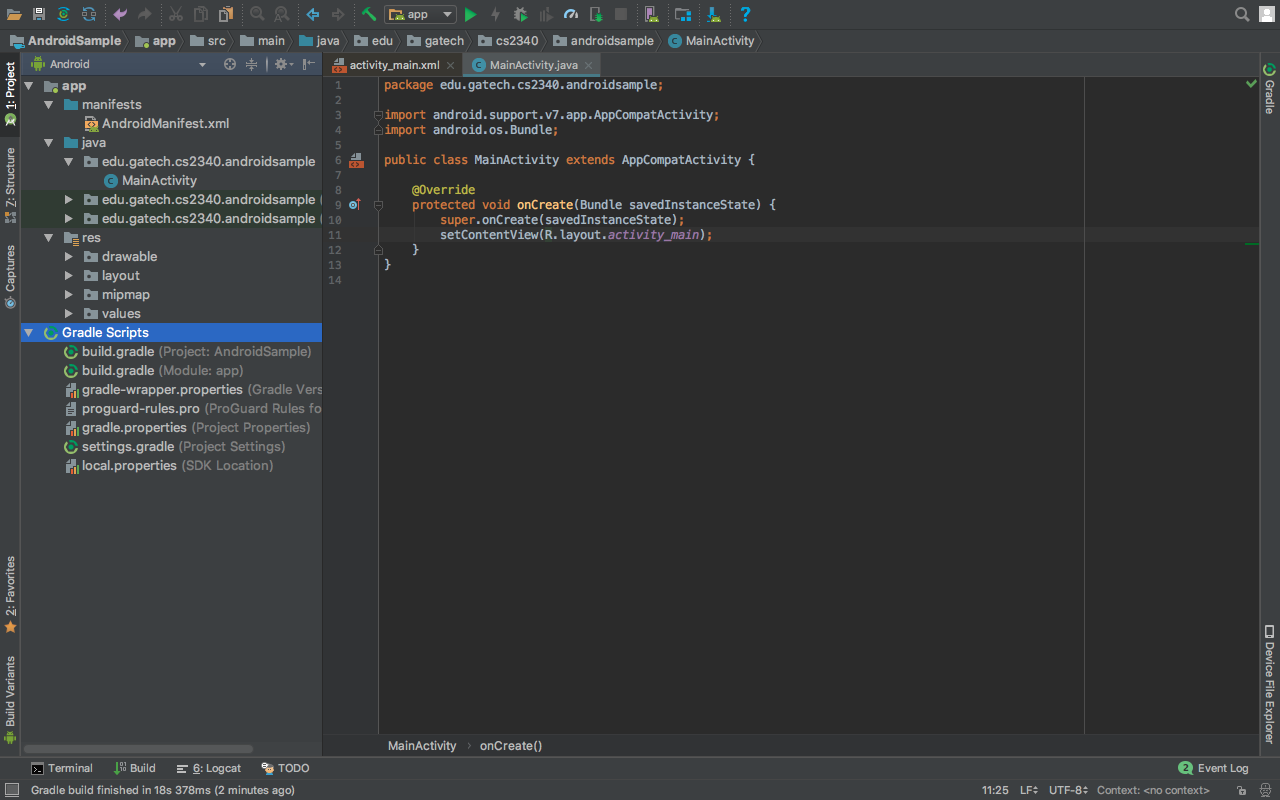
\includegraphics[width=.5\textwidth]{images/ide.png}\end{center}
Select the Project tab at the left of the screen to see your project structure. Here are some important things to observe:
\begin{itemize}
\item \texttt{app > manifests > AndroidManifest.xml} 

This file describes fundamental characteristics of your app, such as the activity that is shown when the app is launched. Manipulation of this file usually happens for you.
\item \texttt{app > java > package name}

This is where your code lives. The package name defaults to being the reverse of the company name you selected followed by the name of your app (e.g. I chose a company name of \texttt{cs2340.gatech.edu} and named my app \texttt{Android Sample}, so the company name that was generated is \texttt{edu.gatech.cs2340.androidsample}).
\item \texttt{MainActivity.java}

In an Android app, different UI screens are organized into activities. These are Java classes that are subclasses of some Android Activity class. The operating system handles the instantiation of your Activities. In this app, the MainActivity that you created when setting up the project is the Activity that is launched when the app is run.
\item \texttt{app > res > layout}

This is where your UI layouts live. These are XML files that define how things are organized on your screen. You will almost always manipulate these using the GUI shown below, and not as raw XML.
\item \texttt{activity\_main.xml}

This is the layout file that corresponds to \texttt{MainActivity.java}.
\item \texttt{Gradle Scripts}

Gradle is the tool that builds your app. Android Studio does a lot of work with these for you, and in practice you will rarely have to manipulate a Gradle script yourself in Android Studio.
\end{itemize}

\section{Running the App}
Now it is time to run your app, which we will do on an emulator. Select \texttt{Run (menu) > Run} or click 
\includegraphics[height=9pt]{images/run.png} in the toolbar. This opens the Select Deployment Target window:
\begin{center}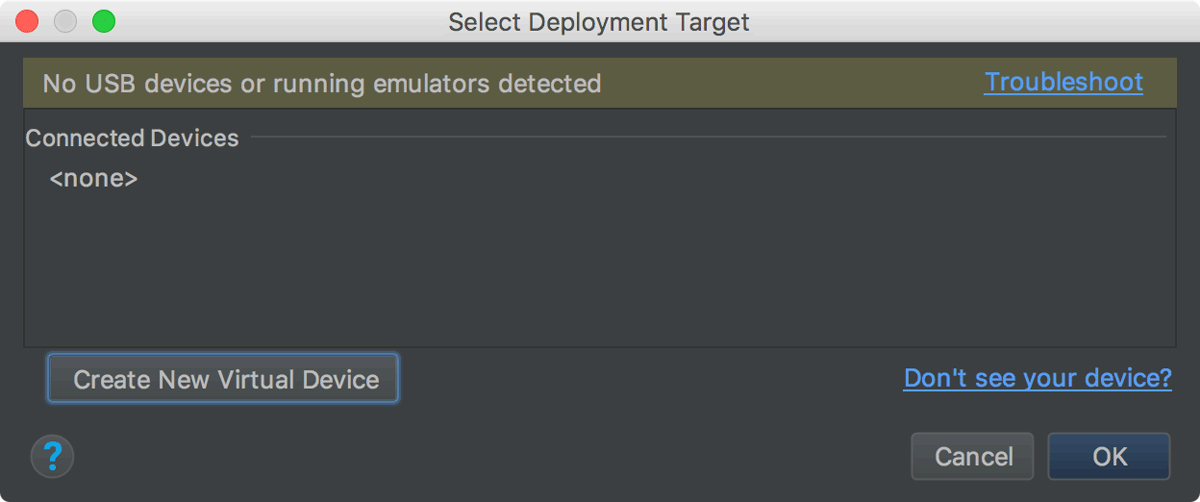
\includegraphics[width=.5\textwidth]{images/select-deploy.png}\end{center}
The first time you do this, click Create New Virtual Device. Select a phone (I usually use the Pixel), and click Next. Now select a system image; for this, select the version with the highest API level. Download it if necessary. On the next screen, rename the device if you wish and click Finish. You should be back in the Select Deployment Target window now. Select the device you created and click OK. After the emulator boots, your app should be running on it:
\begin{center}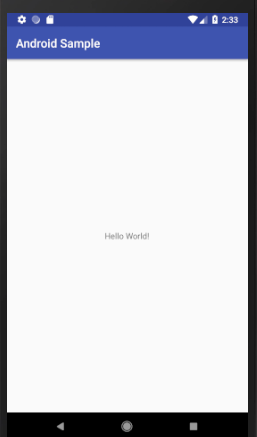
\includegraphics[height=.44\textheight]{images/hello-world.png}\end{center}

\section{Adding Features}
Now that you have a functioning app, it's time to make it do something. First, some setup. Open 
\texttt{app > res > layout > activity\_main.xml}. Click the Project 
\includegraphics[height=9pt]{images/project.png} tab at the left of the screen to hide the Project window if you need more room. If you see the raw XML, click the Design tab near the bottom to switch to the design view. Click 
\includegraphics[height=9pt]{images/show.png} and ensure that Show Constraints is checked, and then make sure that Autoconnect is turned off (it should appear as 
\includegraphics[height=9pt]{images/autoconnect-off.png}). Now, we remove the "Hello World!" \texttt{TextView}. Click on \texttt{TextView - "Hello World!"} in the Component Tree and press delete. The Component Tree window displays the layout's hierarchy of views. The root view of your layout is a \texttt{ConstraintLayout}. This layout positions each view according to constraints to sibling views and the parent layout. Now let's add some views. In the Palette, click Text to display available text controls. Drag a \texttt{TextView} into the design editor and drop it in your layout. The result should look like this:
\begin{center}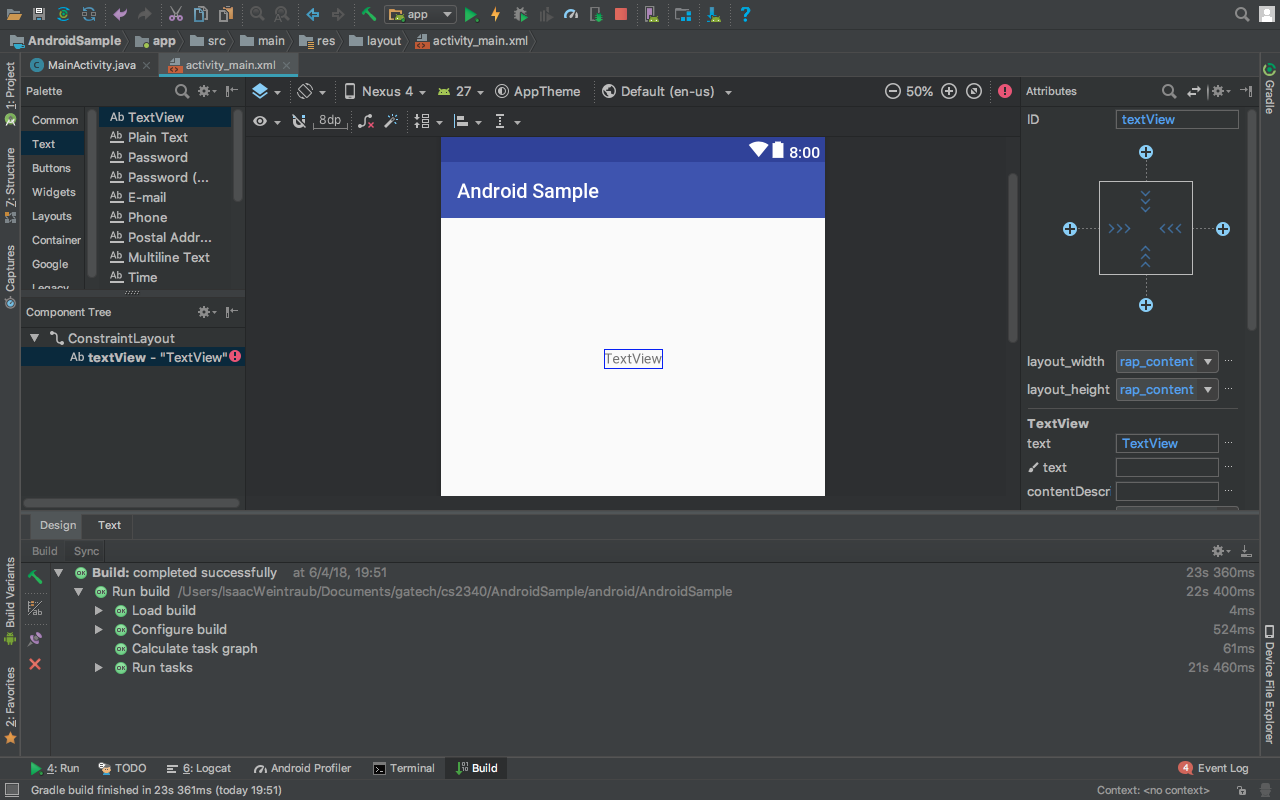
\includegraphics[width=.5\textwidth]{images/add-textview.png}\end{center}
\texttt{TextView} displays text. You will notice that there is a reddish exclamation point near the top right of the editor. This is warning you that the \texttt{TextView} is not constrained and will therefore jump to location $(0,0)$ at runtime unless you constrain it. Add a vertical constraint by clicking on the \texttt{TextView} and dragging upward from the node on top of it to the top of the view, where the \texttt{TextView} will snap upwards. The TextView is now constrained vertically to be a fixed distance from the top of the screen and should look as follows:
\begin{center}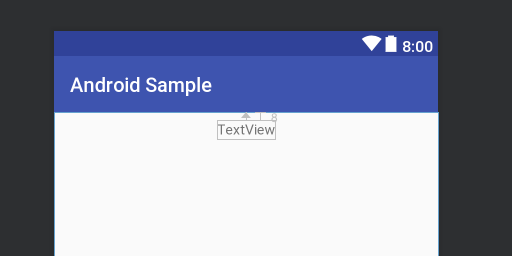
\includegraphics[width=.4\textwidth]{images/textview-vc.png}\end{center}
When the \texttt{TextView} is selected, at the right of your screen there is a panel displaying its attributes. Below the ID attribute, you will see a diagram representing that the \texttt{TextView} is constrained to have a vertical margin of 8 pixels:
\begin{center}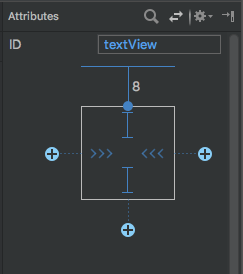
\includegraphics[width=.3\textwidth]{images/vertical-constraint.png}\end{center}
Click on the 8 and change it to 32 pixels. Now center the \texttt{TextView} horizontally by dragging right on the \texttt{TextView}'s right node and then left on its left node. The next thing to do is make the \texttt{TextView} a little more interesting. In the Attributes panel, replace the value of the \texttt{text} attribute with "Welcome to CS 2340!" Below this, you can change the text's font, size, color, and more. Choose a color that looks appealing, and increase the font size to 24 point. If the bottom of the text is cut off, change the \texttt{layout\_height} attribute's value to "wrap\_content". Your layout should now appear as follows:
\begin{center}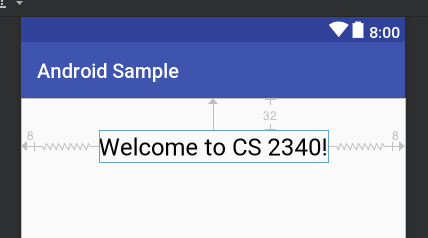
\includegraphics[width=.4\textwidth]{images/textview-fancy.png}\end{center}
Next, add a Plain Text and a Button from the palette. The Plain Text is an \texttt{EditText}, which accepts text input. Constrain both of these to be 32 pixels below the \texttt{TextView}, change the Button's \texttt{text} attribute to say "Do Something", and constrain the Button to be 16 pixels from the right of the screen. Now make the text box's size flexible. Do this by clicking on the \texttt{EditText}'s 
\includegraphics[height=9pt]{images/fixed.png} in the Attributes panel until it appears as 
\includegraphics[height=9pt]{images/match.png}. This signifies that the text box will stretch horizontally to fill available space. Constrain the text box as before so that it is 16 pixels from the left of the screen and 8 pixels to the left of the Button, and your layout should look similar to this:
\begin{center}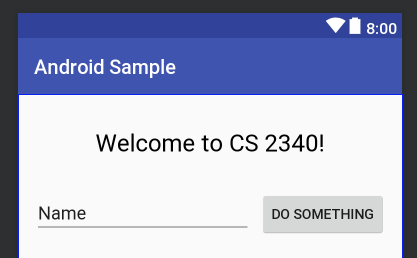
\includegraphics[width=.4\textwidth]{images/ui.png}\end{center}
As of right now, the button does nothing. Let's change that. Open \texttt{MainActivity.java}. If you have used IntelliJ before, this should be familiar to you, since Android Studio is essentially IntelliJ set up to do Android development. Below the \texttt{onCreate()} method, add the \texttt{doSomething()} method shown below:
\begin{lstlisting}[language=Java]
/* 
 * This method will be called when the button is pressed.
 * add JavaDocs to your heart's content
 */
public void doSomething(View view) {
    Intent intent = new Intent(this, NextActivity.class);
    EditText text = (EditText) findViewById(R.id.editText);
    String name = text.getText().toString();
    intent.putExtra("NAME", name);
    startActivity(intent);
}
\end{lstlisting}
While coding, when you use a class that has not been imported yet, perhaps \texttt{View}, Android Studio will alert you of this fact and will suggest that you import \texttt{android.view.View}. Press Alt/Option-Enter to accept this suggestion. There are several important things happening in this method:
\begin{itemize}
\item Method signature. In order to be compatible with the Button's \texttt{onClick} attribute, a method needs to have \texttt{public} access, return \texttt{void}, and take a \texttt{View} (the \texttt{View} object that was clicked) as its only parameter.
\item Interaction with UI Views. \texttt{findViewById()} locates a \texttt{View} from the id you specify. You can change the id of a view in the layout file by changing the \texttt{id} property. \texttt{R} is an auto-generated file that keeps track of Views as well as other resources.
\item Intents. An \texttt{Intent} binds separate components, such as activities. It represents an app's "intent to do something". Here you have an \texttt{Intent} for starting a new activity, which you will create in a moment. The \texttt{Intent} constructor takes a \texttt{Context}, for which we use \texttt{this} since activity classes are subclasses of \texttt{Context}, as well as the \texttt{Class} of the component to which the \texttt{Intent} is being delivered. The \texttt{putExtra()} method is used to add information to an \texttt{Intent}. An \texttt{Intent} can carry data in key-value pairs, or extras.
\end{itemize}
Go back to \texttt{activity\_main.xml} and set the Button's \texttt{onClick} property to \texttt{doSomething} so that the Button calls \texttt{doSomething()} when it is clicked. Now you need to create the \texttt{NextActivity}. In the Project window, right click the \texttt{app} folder and select \texttt{New > Activity > Empty Activity}. Name this activity NextActivity, leave everything else at its default value, and click Finish. Android Studio has created the \texttt{NextActivity.java} file, the corresponding texttt{activity\_next.xml} layout, and registered the activity in \texttt{AndroidManifest.xml}. At this point you should be able to run the app and the button will launch the next activity, but the second activity is not especially interesting:
\begin{center}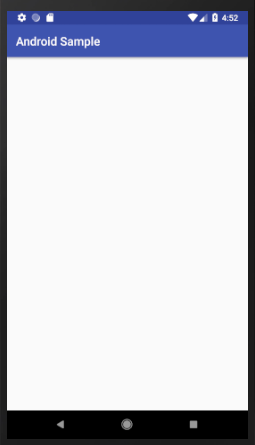
\includegraphics[width=.4\textwidth]{images/wauw.png}\end{center}
Now you will add something moderately interesting to the next activity. Open the layout file that corresponds to it (\texttt{app > res > layout > activity\_next.xml}), and add a TextView. Center it horizontally and vertically, and alter the style of the text as desired. Now add some code to \texttt{NextActivity}'s \texttt{onCreate()} method to display a message:
\begin{lstlisting}[language=Java]
@Override
protected void onCreate(Bundle savedInstanceState) {
    super.onCreate(savedInstanceState);
    setContentView(R.layout.activity_next);
    
    // You will need to add the code below.
    Intent intent = getIntent();
    String name = intent.getStringExtra("NAME");
    TextView textView = findViewById(R.id.textView2);
    textView.setText(embellish(name));
}
\end{lstlisting}
And the \texttt{embellish()} method:
\begin{lstlisting}[language=Java]
private String embellish(String name) {
    String ret = "";
    for (int i = 0; i < name.length(); i++) {
        for (int j = 0; j < name.length(); j++) {
            ret += name.charAt((j - i + name.length()) % name.length());
        }
        if (i != name.length() - 1) {
            ret += "\n";
        }
    }
    return ret;
}
\end{lstlisting}
In \texttt{onCreate()}, you get the \texttt{Intent} that started this activity and extract the value of the NAME extra. You then find the \texttt{TextView} you put in the layout, and set its text. \texttt{embellish()} is regular Java that you could have seen in CS 1331. Now, you can run the app, and it should become clear how \texttt{embellish()} operates: 
\begin{center}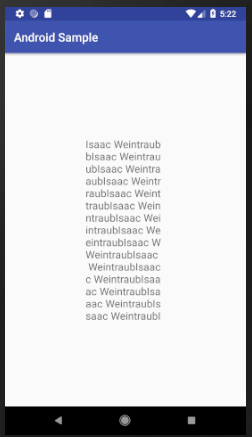
\includegraphics[width=.4\textwidth]{images/finished.png}\end{center}
And with that, you have just built an Android app!

\section{Further Information}
In your Android development endeavors, you may find the following resources useful:
\begin{itemize}
\item Android development tutorials: \url{https://developer.android.com/guide/} 
\item Android API reference: \url{https://developer.android.com/reference/}
\item Guide to using Android Studio: \url{https://developer.android.com/studio/intro/} 
\item Java 7 API specification: \url{https://docs.oracle.com/javase/7/docs/api/} 
\item Java 8 API specification: \url{https://docs.oracle.com/javase/8/docs/api/}
\item Sample \texttt{.gitignore} for Android projects:\\ \url{https://github.com/github/gitignore/blob/master/Android.gitignore}
\item Source code for this app: \url{https://github.com/IsaacWeintraub/AndroidSample} 
\end{itemize}
\end{document}